\chapter{Charting}
\label{ch:charting}

\ccprod{} draws three kinds of picture --- bars, a line and a pie --- all of
them of the numbers in one column, and any of them can be saved to the card as
a picture file. It is not a charting package. It is the small honest version of
the feature that made spreadsheets worth buying, and it takes one command and
no configuration at all.

\section{Drawing a chart}
\index{chart}

Put the cursor in the column you want to chart, on the first row of it, and
choose one of the three commands on the \menupath{Chart} menu.

\begin{cctable}{Command}{Draws}{2.2in}{2.62in}
\menupath{Chart > Bars} & A bar chart \\
\menupath{Chart > Line} & A line chart \\
\menupath{Chart > Pie} & A pie chart \\
\end{cctable}

None of them has a keyboard shortcut, and none has any options. The chart fills
the screen. Press \key{S} to save it; press anything else to go straight back to
the worksheet.

\begin{ccfigure}
\begin{tikzpicture}[x=1pt,y=-1pt]
  \definecolor{cbar}{HTML}{2E2C9B}\definecolor{cgrey}{HTML}{B2B2B2}
  % the screen: 640x240 bitmap, shown here at 300pt wide
  \fill[black] (0,0) rectangle (300,124);
  \fill[x16mgrey] (0,0) rectangle (300,9);
  \node[anchor=base west,font=\ttfamily\fontsize{6}{7}\selectfont,text=white]
    at (3,6.6) {Column B};
  % axis figures, blitted into the picture
  \node[anchor=base west,font=\ttfamily\fontsize{5.4}{6.4}\selectfont,
        text=white] at (2,20) {8400};
  \node[anchor=base west,font=\ttfamily\fontsize{5.4}{6.4}\selectfont,
        text=white] at (2,101) {0};
  % zero line
  \fill[cgrey] (34,101) rectangle (298,102.5);
  % six bars: ten cells wide, stepped eleven cells apart
  \foreach \i/\hh in {0/83,1/30,2/4.2,3/2.3,4/11.3,5/2.1}{
    \fill[cbar] ({34+\i*41.3},{101-\hh}) rectangle ++(37.5,\hh);
  }
  % labels, blitted under the plot -- ten characters each, so these all fit
  \foreach \i/\n in {0/Salaries,1/Rent,2/Power,3/Supplies,4/Travel,
                     5/Insurance}{
    \node[anchor=base west,font=\ttfamily\fontsize{5.2}{6.2}\selectfont,
          text=white] at ({35+\i*41.3},110) {\n};
  }
  \fill[x16mgrey] (2,113) rectangle (68,121);
  \node[anchor=base west,font=\ttfamily\fontsize{6}{7}\selectfont,text=white]
    at (3,119.5) {Any key, S saves};
  \draw[ccink,line width=0.7pt] (0,0) rectangle (300,124);
\end{tikzpicture}
\caption{\menupath{Chart > Bars} on column \cellref{B}, with column \cellref{A}
supplying the labels}
\label{fig:chart}
\end{ccfigure}

\begin{ccnote}
Everything you see on a chart --- the bars, the axis figures, the labels, the
pie's key --- is part of one picture, not text laid over it. That is what makes
it possible to save the whole thing, and it is why the letters on a chart are
smaller and finer than the ones in the worksheet.
\end{ccnote}

\section{What gets charted}

The same rules apply to all three kinds.

\begin{ccsteps}
\item \textbf{The cursor's column}, and only that column. There is no way to
chart two series together.
\item \textbf{From the cursor's row downwards}, to the end of the used range.
\item \textbf{At most sixteen values.} The real limit is how many can be
labelled --- four characters of screen for each --- and on an eighty-column
display that works out at sixteen. A longer column is charted from the cursor
down and simply stops. To chart the rest, move the cursor further down and run
the command again.
\item \textbf{Numbers only.} Text and \msg{TRUE}/\msg{FALSE} cells are skipped
rather than counted as zero --- which is what makes it safe to put the cursor on
a heading row --- and so are empty cells. A formula is charted if its result is
a number.
\end{ccsteps}

\begin{ccnote}
The chart reads each cell's stored value, not what the worksheet shows. A
currency column charts correctly even though what is on screen reads
\lit{\$8400.00}.
\end{ccnote}

The title line names the column: \msg{Column B}. The bottom of the screen says
\msg{Any key, S saves}. If there are no numbers at all from the cursor down,
\ccprod{} says \msg{No numbers} and waits for a key --- the worksheet is not
cleared off the screen until the program knows it has something to draw.

\section{The labels}
\index{chart!labels}

Labels come from \textbf{the column immediately to the left} of the one being
charted, on the same rows.

So a table laid out with names in column \cellref{A} and figures in column
\cellref{B} charts with its names already in place, which is the layout worth
building for. If the cursor is in column \cellref{A} there is nothing to the
left of it and the chart is drawn without labels.

A label is cut off at the width it has --- the width of its bar on a bar chart,
twelve characters in the pie's key.

\section{Bars and lines}
\index{chart!bar}\index{chart!line}

Both are drawn against the same scale, with the same axis, and differ only in
what fills the plot: bars are solid blue blocks, and a line is a red trace with
a thicker mark at each value.

\begin{ccsteps}
\item \textbf{The scale always includes zero}, whether or not any of the data is
near it. A column running from 90 to 100 draws bars that are nearly full height,
not a row of stubs differing in the last pixel. A chart whose baseline is not
zero exaggerates, and this one is small enough already.
\item The top and bottom of the scale are printed up the left-hand edge.
\item A zero line is drawn across the plot. On a bar chart \textbf{negative
values hang below it}.
\item A column in which every value is the same draws every bar at full height.
\end{ccsteps}

\begin{ccnote}
The line joining two points is a vertical step rather than a true diagonal. At a
dozen points across the screen that is very close to what a diagonal would come
to anyway, and it costs a great deal less arithmetic on an eight-megahertz
processor.
\end{ccnote}

\section{Pie charts}
\index{chart!pie}

\menupath{Chart > Pie} draws a circle divided into slices in proportion to the
values, with a key beside it giving each slice's label and its share as a
whole-number percentage.

\begin{ccfigure}
\begin{tikzpicture}[x=1pt,y=-1pt]
  \definecolor{pieA}{HTML}{2E2C9B}\definecolor{pieB}{HTML}{EDF171}
  \definecolor{pieC}{HTML}{813338}\definecolor{pieD}{HTML}{56AC4D}
  \definecolor{pieE}{HTML}{75CEC8}\definecolor{pieF}{HTML}{8E3C97}
  \fill[black] (0,0) rectangle (300,124);
  \fill[x16mgrey] (0,0) rectangle (300,9);
  \node[anchor=base west,font=\ttfamily\fontsize{6}{7}\selectfont,text=white]
    at (3,6.6) {Column B};
  \begin{scope}[shift={(85,62)}]
    \foreach \a/\b/\c in {0/223/pieA,223/303/pieB,303/314/pieC,
                          314/320/pieD,320/350/pieE,350/360/pieF}{
      \fill[\c] (0,0) -- (\a:44pt) arc[start angle=\a,end angle=\b,radius=44pt]
        -- cycle;
    }
  \end{scope}
  \foreach \i/\n/\p/\c in {0/Salaries/62/pieA,1/Rent/22/pieB,2/Power/3/pieC,
                           3/Supplies/1/pieD,4/Travel/8/pieE,
                           5/Insurance/1/pieF}{
    \fill[\c] (190,{20+\i*10}) rectangle ++(6,6);
    \node[anchor=base west,font=\ttfamily\fontsize{5.4}{6.4}\selectfont,
          text=white] at (201,{25.5+\i*10}) {\n};
    \node[anchor=base east,font=\ttfamily\fontsize{5.4}{6.4}\selectfont,
          text=white] at (292,{25.5+\i*10}) {\p\%};
  }
  \fill[x16mgrey] (2,113) rectangle (68,121);
  \node[anchor=base west,font=\ttfamily\fontsize{6}{7}\selectfont,text=white]
    at (3,119.5) {Any key, S saves};
  \draw[ccink,line width=0.7pt] (0,0) rectangle (300,124);
\end{tikzpicture}
\caption{\menupath{Chart > Pie}, with its key drawn into the picture beside it}
\label{fig:pie}
\end{ccfigure}

\begin{ccsteps}
\item \textbf{Negative values are dropped}, not charted as anything --- a slice
cannot be less than nothing. The percentages are shares of the total of what is
left, so a column with negatives in it will not give the shares you expect.
\item If every value is negative or zero there is no total to take shares of,
and \ccprod{} says \msg{No numbers}.
\item Percentages are whole numbers, rounded down, so they will not always add
up to 100.
\item Slice colours cycle through six and then repeat. With more than six values
two slices will share a colour; the key is what tells them apart.
\end{ccsteps}

\section{Saving a chart}
\index{chart!saving}\index{CHART.BMP}

Press \key{S} while the chart is on screen.

\ccprod{} writes the picture to the card as \fname{CHART.BMP}, returns to the
worksheet, and says so on the bottom line:

\begin{ccfigure}
\ccscreenscale{1.5}
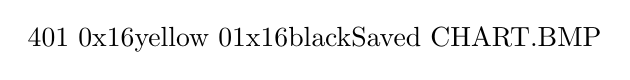
\begin{tikzpicture}
\node[inner sep=0pt,anchor=north west] (sv) at (0,0) {%
\ccscreenbegin{40}{1}
  \ccfillrow{0}{x16yellow}
  \cctext{0}{1}{x16black}{Saved~CHART.BMP}
\ccscreenend
};
\end{tikzpicture}
\caption[The message after S]{The message after \key{S}}
\label{fig:chartsaved}
\end{ccfigure}

If it cannot be written --- a full card, a write-protected one, no card at all
--- the message is \msg{Could not write CHART.BMP} instead. Either way the
message stays until the next time the screen is redrawn.

\begin{cctable}{About the file}{ }{1.6in}{3.22in}
Name & \fname{CHART.BMP}, always. You are not asked for one. \\
Format & Windows \fname{.BMP}, 640 by 480 pixels, sixteen colours. \\
Size & About 150K. \\
Read by & Anything that opens a \fname{.BMP} --- every paint program, every
image viewer, every word processor. \\
\end{cctable}

\begin{cccaution}
\textbf{The name is always \fname{CHART.BMP}, so each save overwrites the last
one.} If you want to keep two charts, copy or rename the first before drawing
the second.
\end{cccaution}

\begin{ccnote}
\fname{.BMP} rather than anything smaller because it is the one picture format
this program can write honestly: the others need compression, and \ccprod{}
carries only the code to \emph{un}compress. The saved file is bigger than it
needs to be and completely standard.

It is also twice the height of the picture the machine draws. \ccprod{} charts
into a bitmap 640 by 240, and shows it on a display running at half vertical
scale --- so a dot on that bitmap is one pixel wide and two tall, and the pie is
swept as an ellipse precisely so that the glass shows a circle. A file has no
such display behind it, and every program that opens one assumes square dots.
Each row is therefore written twice, which puts the scaling into the file and
makes it open as the circle you were looking at.
\end{ccnote}

\section{What a chart is not}

\begin{ccsteps}
\item It cannot be printed, and it is not stored in the workbook --- neither
\fname{.X16S} nor \fname{.XLSX} carries it. \fname{CHART.BMP} is the only record
of one.
\item There is no stacked, scatter or area chart.
\item There is no title you can set, no axis labelling, no colour choice and no
scaling option. The pie's key is the only legend there is.
\item A chart is a picture of the numbers as they were when you drew it. It does
not update, because it does not persist.
\end{ccsteps}
